\documentclass[]{article}
\usepackage{lmodern}
\usepackage{amssymb,amsmath}
\usepackage{ifxetex,ifluatex}
\usepackage{fixltx2e} % provides \textsubscript
\ifnum 0\ifxetex 1\fi\ifluatex 1\fi=0 % if pdftex
  \usepackage[T1]{fontenc}
  \usepackage[utf8]{inputenc}
\else % if luatex or xelatex
  \ifxetex
    \usepackage{mathspec}
    \usepackage{xltxtra,xunicode}
  \else
    \usepackage{fontspec}
  \fi
  \defaultfontfeatures{Mapping=tex-text,Scale=MatchLowercase}
  \newcommand{\euro}{€}
\fi
% use upquote if available, for straight quotes in verbatim environments
\IfFileExists{upquote.sty}{\usepackage{upquote}}{}
% use microtype if available
\IfFileExists{microtype.sty}{%
\usepackage{microtype}
\UseMicrotypeSet[protrusion]{basicmath} % disable protrusion for tt fonts
}{}
\usepackage[margin=1in]{geometry}
\usepackage{color}
\usepackage{fancyvrb}
\newcommand{\VerbBar}{|}
\newcommand{\VERB}{\Verb[commandchars=\\\{\}]}
\DefineVerbatimEnvironment{Highlighting}{Verbatim}{commandchars=\\\{\}}
% Add ',fontsize=\small' for more characters per line
\usepackage{framed}
\definecolor{shadecolor}{RGB}{248,248,248}
\newenvironment{Shaded}{\begin{snugshade}}{\end{snugshade}}
\newcommand{\KeywordTok}[1]{\textcolor[rgb]{0.13,0.29,0.53}{\textbf{{#1}}}}
\newcommand{\DataTypeTok}[1]{\textcolor[rgb]{0.13,0.29,0.53}{{#1}}}
\newcommand{\DecValTok}[1]{\textcolor[rgb]{0.00,0.00,0.81}{{#1}}}
\newcommand{\BaseNTok}[1]{\textcolor[rgb]{0.00,0.00,0.81}{{#1}}}
\newcommand{\FloatTok}[1]{\textcolor[rgb]{0.00,0.00,0.81}{{#1}}}
\newcommand{\CharTok}[1]{\textcolor[rgb]{0.31,0.60,0.02}{{#1}}}
\newcommand{\StringTok}[1]{\textcolor[rgb]{0.31,0.60,0.02}{{#1}}}
\newcommand{\CommentTok}[1]{\textcolor[rgb]{0.56,0.35,0.01}{\textit{{#1}}}}
\newcommand{\OtherTok}[1]{\textcolor[rgb]{0.56,0.35,0.01}{{#1}}}
\newcommand{\AlertTok}[1]{\textcolor[rgb]{0.94,0.16,0.16}{{#1}}}
\newcommand{\FunctionTok}[1]{\textcolor[rgb]{0.00,0.00,0.00}{{#1}}}
\newcommand{\RegionMarkerTok}[1]{{#1}}
\newcommand{\ErrorTok}[1]{\textbf{{#1}}}
\newcommand{\NormalTok}[1]{{#1}}
\usepackage{graphicx}
\makeatletter
\def\maxwidth{\ifdim\Gin@nat@width>\linewidth\linewidth\else\Gin@nat@width\fi}
\def\maxheight{\ifdim\Gin@nat@height>\textheight\textheight\else\Gin@nat@height\fi}
\makeatother
% Scale images if necessary, so that they will not overflow the page
% margins by default, and it is still possible to overwrite the defaults
% using explicit options in \includegraphics[width, height, ...]{}
\setkeys{Gin}{width=\maxwidth,height=\maxheight,keepaspectratio}
\ifxetex
  \usepackage[setpagesize=false, % page size defined by xetex
              unicode=false, % unicode breaks when used with xetex
              xetex]{hyperref}
\else
  \usepackage[unicode=true]{hyperref}
\fi
\hypersetup{breaklinks=true,
            bookmarks=true,
            pdfauthor={Abbas Rizvi},
            pdftitle={STA 546 - Homework 2},
            colorlinks=true,
            citecolor=blue,
            urlcolor=blue,
            linkcolor=magenta,
            pdfborder={0 0 0}}
\urlstyle{same}  % don't use monospace font for urls
\setlength{\parindent}{0pt}
\setlength{\parskip}{6pt plus 2pt minus 1pt}
\setlength{\emergencystretch}{3em}  % prevent overfull lines
\setcounter{secnumdepth}{0}

%%% Use protect on footnotes to avoid problems with footnotes in titles
\let\rmarkdownfootnote\footnote%
\def\footnote{\protect\rmarkdownfootnote}

%%% Change title format to be more compact
\usepackage{titling}

% Create subtitle command for use in maketitle
\newcommand{\subtitle}[1]{
  \posttitle{
    \begin{center}\large#1\end{center}
    }
}

\setlength{\droptitle}{-2em}
  \title{STA 546 - Homework 2}
  \pretitle{\vspace{\droptitle}\centering\huge}
  \posttitle{\par}
  \author{Abbas Rizvi}
  \preauthor{\centering\large\emph}
  \postauthor{\par}
  \predate{\centering\large\emph}
  \postdate{\par}
  \date{March 9, 2016}



\begin{document}

\maketitle


\section{Problem 1}\label{problem-1}

Principal component analysis (PCA) is an exploratory technique that is
useful when examining patterns in high-dimensional datasets. PCA uses an
orthogonal transformation to convert a set of observations into mutually
uncorrelated, ordered variables known as principal components (PC). PCA
transforms the data such that the first principal component
(\texttt{PC1}) captures the largest variance possible. The successive
prinicpal components have the highest variance possible under the
condition that the component is orthogonal to the preceding components.
Generally, if the sample variances of the first few PCs are large, and
the remaining set of PCs are small, the small PCs can be viewed as
having low variance relative to other variables, and can be omitted form
the analysis.

PCA was implemented on the \texttt{SwissBankNotes} dataset. The
\texttt{SwissBankNotes} dataset was loaded into the \texttt{R} global
environment.

\begin{Shaded}
\begin{Highlighting}[]
\KeywordTok{load}\NormalTok{(}\StringTok{"SwissBankNotes.rdata"}\NormalTok{)}
\end{Highlighting}
\end{Shaded}

\texttt{SwissDataNotes} consists of six variables of measurements
conducted on old Swiss 1,000-franc bank notes, with the first 100 rows
consisting of genuine notes and the second 100 are counterfeit. The
measurement variables can be seen here:

\begin{Shaded}
\begin{Highlighting}[]
\KeywordTok{colnames}\NormalTok{(SwissBankNotes)}
\end{Highlighting}
\end{Shaded}

\begin{verbatim}
## [1] "length"       "height.left"  "height.right" "inner.lower" 
## [5] "inner.upper"  "diagonal"
\end{verbatim}

\begin{Shaded}
\begin{Highlighting}[]
\NormalTok{SwissBankNotes <-}\StringTok{ }\KeywordTok{cbind}\NormalTok{(SwissBankNotes,}
                        \KeywordTok{as.factor}\NormalTok{(}\KeywordTok{c}\NormalTok{(}\KeywordTok{rep}\NormalTok{(}\StringTok{"genuine"}\NormalTok{,}\DecValTok{100}\NormalTok{), }\KeywordTok{rep}\NormalTok{(}\StringTok{"counterfeit"}\NormalTok{, }\DecValTok{100}\NormalTok{))))}
\KeywordTok{colnames}\NormalTok{(SwissBankNotes)[}\DecValTok{7}\NormalTok{] <-}\StringTok{ "class"}
\end{Highlighting}
\end{Shaded}

The dataset was stratified into three different groups: (1) the 100
genuine notes only, (2) the 100 counterfeit notes only, and (3) the
complete dataset. \texttt{stats::prcomp} was used to implement PCA
across groups and return them as a \texttt{prcomp} object. Typically,
the data is centered for PCA, such that we let \(x_{i}\) be a column in
\texttt{SwissBankNotes} and we subtract by the \texttt{colMeans},
\(x^{*}_{i} = x_{i} - \bar{x}\), where \(x^{*}_{i}\) is the centered
variable. Colloquially, this means that the column-wise empirical mean
is equal to zero. This is necessary for PCA to ensure that PC1
characterizes the maximum variance.

We conduct PCA using singular value decomposition of the centered
covariance matrix (\texttt{prcomp(x, scale = FALSE)}) and the
correlation matrix (\texttt{prcomp(x, scale = TRUE)}). The decision to
implement scaling is subjective and may be useful to explore both
options depending on the data at hand. For this exercise we will only
used scaled data. PCA is quite sensitive to scaling of variables. PCA is
less arbitrary when scaled by normalization (via using a correlation
matrix or normalizing by mean-squared error (MSE)).

We investigated the proportion of variance captured by PCA by summary
statistics or visually through screeplots and/or biplots. Explained
proportion of variance can also be obtained dividing the eigenvalues of
the correlation matrix by the sum of all the eigenvalues of the
correlation matrix.

\texttt{stats::screeplot} plots the variances against ordered PCs from
an object of class \texttt{prcomp}. The \texttt{biplot} is an enhanced
scatterplot that uses both points and vectors to represent a structure.
The biplots shown in this exercise will only be \texttt{PC1} vs.
\texttt{PC2}.

\begin{Shaded}
\begin{Highlighting}[]
\NormalTok{genuine <-}\StringTok{ }\KeywordTok{prcomp}\NormalTok{(SwissBankNotes[SwissBankNotes$class ==}\StringTok{ 'genuine'}\NormalTok{,-}\DecValTok{7}\NormalTok{], }\DataTypeTok{scale=}\OtherTok{TRUE}\NormalTok{) }
\NormalTok{counterfeit <-}\StringTok{ }\KeywordTok{prcomp}\NormalTok{(SwissBankNotes[SwissBankNotes$class ==}\StringTok{ 'counterfeit'}\NormalTok{,-}\DecValTok{7}\NormalTok{], }\DataTypeTok{scale=}\OtherTok{TRUE}\NormalTok{)}
\NormalTok{complete <-}\StringTok{ }\KeywordTok{prcomp}\NormalTok{(SwissBankNotes[,-}\DecValTok{7}\NormalTok{], }\DataTypeTok{scale=}\OtherTok{TRUE}\NormalTok{)}

\KeywordTok{summary}\NormalTok{(genuine)}
\end{Highlighting}
\end{Shaded}

\begin{verbatim}
## Importance of components:
##                           PC1    PC2    PC3     PC4     PC5     PC6
## Standard deviation     1.4845 1.3026 0.9827 0.76348 0.57156 0.47340
## Proportion of Variance 0.3673 0.2828 0.1610 0.09715 0.05445 0.03735
## Cumulative Proportion  0.3673 0.6501 0.8111 0.90820 0.96265 1.00000
\end{verbatim}

\begin{Shaded}
\begin{Highlighting}[]
\KeywordTok{summary}\NormalTok{(counterfeit)}
\end{Highlighting}
\end{Shaded}

\begin{verbatim}
## Importance of components:
##                           PC1    PC2    PC3    PC4     PC5     PC6
## Standard deviation     1.3915 1.3285 0.9941 0.8823 0.56755 0.45840
## Proportion of Variance 0.3227 0.2941 0.1647 0.1297 0.05368 0.03502
## Cumulative Proportion  0.3227 0.6169 0.7816 0.9113 0.96498 1.00000
\end{verbatim}

\begin{Shaded}
\begin{Highlighting}[]
\KeywordTok{summary}\NormalTok{(complete)}
\end{Highlighting}
\end{Shaded}

\begin{verbatim}
## Importance of components:
##                           PC1    PC2    PC3     PC4     PC5     PC6
## Standard deviation     1.7163 1.1305 0.9322 0.67065 0.51834 0.43460
## Proportion of Variance 0.4909 0.2130 0.1448 0.07496 0.04478 0.03148
## Cumulative Proportion  0.4909 0.7039 0.8488 0.92374 0.96852 1.00000
\end{verbatim}

Looking at the summary statistics, we can see that all three groups show
that \texttt{PC1} has the greatest proportion of variance, followed by
\texttt{PC2}, and so on. This finding supports our convenient property
that maximal amount of variance is being captured in the preceding PC.

\begin{figure}[htbp]
\centering
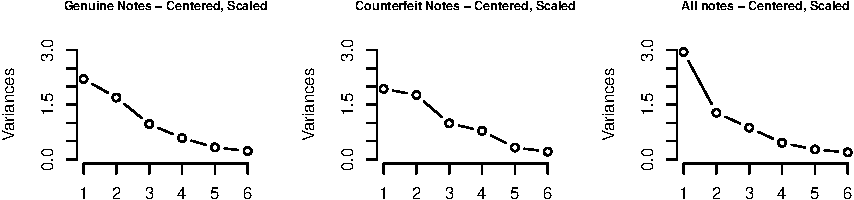
\includegraphics{sta546_hw2_files/figure-latex/unnamed-chunk-4-1.pdf}
\caption{Screeplots of SwissBankNote Groups}
\end{figure}

When intepreting a screeplot, if two data points have a noticeable
separation (decrease in value along y-axis) in the succeeding data point
along the x-axis, we can call this an ``elbow''. An ideal ``elbow'' can
be seen in the PCA of the complete datset (Figure 1, right panel), where
a visible degree of separation between the \texttt{PC1} and \texttt{PC2}
is present. The genuine (Figure 1, left panel) and counterfeit (Figure
1, middle panel) groups alone, do not have profound elbows. This could
indicate that we may want to investigate the unscaled data.

We use biplots to explore samples and variables of a data matrix
graphically. The axes of biplots are a pair of PCs. The biplot uses
points to represent the observations on the PC. Observations with
similar variance patterns will cluster in the same spatial area and have
similar scores on the PC. Differing clusters along these principal
components can be intrepreted as having differing variance patterns.
Biplots also use vectors to illustrate the spatial relationship that the
variables have with the points. In other words, the vectors point away
from the origin in some direction and length and are labeled by a
variable that it is most represented by.

The helper function \texttt{ggbiplot} was written to plot
\href{https://github.com/vqv/ggbiplot}{ggbiplot}, which uses the package
\texttt{ggplot2} as it's source for visualization.

\begin{Shaded}
\begin{Highlighting}[]
\KeywordTok{require}\NormalTok{(devtools)}
\KeywordTok{require}\NormalTok{(ggbiplot)}
\NormalTok{gbiplots <-}\StringTok{ }\NormalTok{function(x, components, groups, legend.position)\{}
        \NormalTok{g <-}\StringTok{ }\KeywordTok{ggbiplot}\NormalTok{(x, }\DataTypeTok{obs.scale =} \DecValTok{1}\NormalTok{, }\DataTypeTok{var.scale =} \DecValTok{1}\NormalTok{, }\DataTypeTok{ellipse =} \OtherTok{TRUE}\NormalTok{, }\DataTypeTok{circle=}\OtherTok{FALSE}\NormalTok{,}
                      \DataTypeTok{choice =} \NormalTok{components, }\DataTypeTok{groups=}\NormalTok{groups)}
        \NormalTok{g <-}\StringTok{ }\NormalTok{g +}\StringTok{ }\KeywordTok{scale_color_discrete}\NormalTok{(}\DataTypeTok{name =} \StringTok{''}\NormalTok{)}
        \NormalTok{g <-}\StringTok{ }\NormalTok{g +}\StringTok{ }\KeywordTok{theme}\NormalTok{(}\DataTypeTok{legend.direction =} \StringTok{'horizontal'}\NormalTok{, }\DataTypeTok{legend.position =} \NormalTok{legend.position)}
        \KeywordTok{print}\NormalTok{(g)}
\NormalTok{\}}
\end{Highlighting}
\end{Shaded}

\begin{Shaded}
\begin{Highlighting}[]
\KeywordTok{gbiplots}\NormalTok{(genuine, }\DataTypeTok{components=}\KeywordTok{c}\NormalTok{(}\DecValTok{1}\NormalTok{,}\DecValTok{2}\NormalTok{), }\DataTypeTok{groups=}\OtherTok{FALSE}\NormalTok{, }\DataTypeTok{legend.position =} \StringTok{"none"}\NormalTok{)}
\end{Highlighting}
\end{Shaded}

\begin{figure}[htbp]
\centering
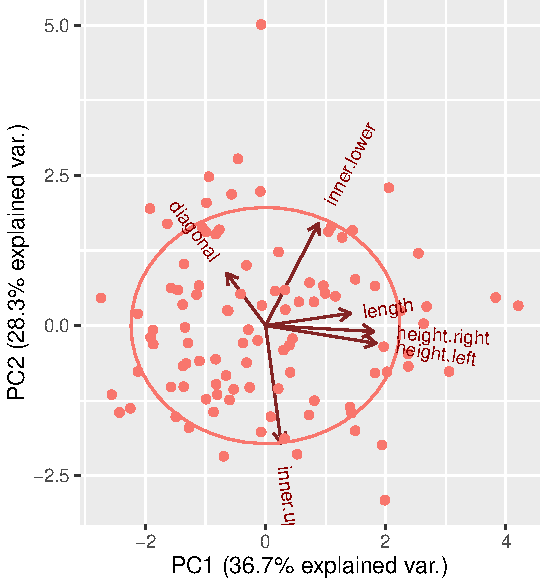
\includegraphics{sta546_hw2_files/figure-latex/unnamed-chunk-6-1.pdf}
\caption{Genuine SwissBankNotes Biplot}
\end{figure}

\begin{Shaded}
\begin{Highlighting}[]
\KeywordTok{gbiplots}\NormalTok{(counterfeit, }\DataTypeTok{components=}\KeywordTok{c}\NormalTok{(}\DecValTok{1}\NormalTok{,}\DecValTok{2}\NormalTok{), }\DataTypeTok{groups=}\OtherTok{FALSE}\NormalTok{, }\DataTypeTok{legend.position =} \StringTok{"none"}\NormalTok{)}
\end{Highlighting}
\end{Shaded}

\begin{figure}[htbp]
\centering
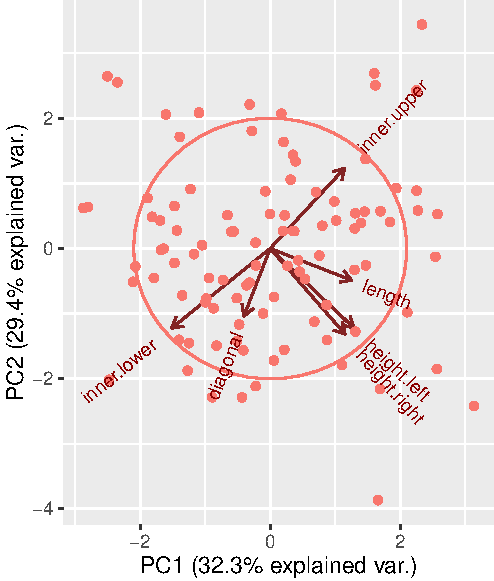
\includegraphics{sta546_hw2_files/figure-latex/unnamed-chunk-6-2.pdf}
\caption{Counterfeit SwissBankNotes Biplot}
\end{figure}

\begin{Shaded}
\begin{Highlighting}[]
\KeywordTok{gbiplots}\NormalTok{(complete, }\DataTypeTok{components=}\KeywordTok{c}\NormalTok{(}\DecValTok{1}\NormalTok{,}\DecValTok{2}\NormalTok{), }\DataTypeTok{groups=}\NormalTok{SwissBankNotes$class, }\DataTypeTok{legend.position=}\StringTok{"top"}\NormalTok{)}
\end{Highlighting}
\end{Shaded}

\begin{figure}[htbp]
\centering
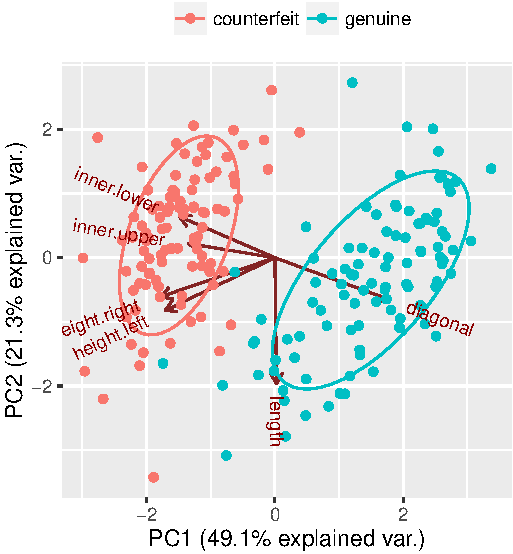
\includegraphics{sta546_hw2_files/figure-latex/unnamed-chunk-6-3.pdf}
\caption{Complete SwissBankNotes Biplot}
\end{figure}

The biplots of the three different groups (genuine alone, counterfeit
alone, or both groups of bank notes) can be see in Figures 2-4,
respectively.

The first 2 PCs plotted against each other for Genuine bank notes can be
seen in Figure 2. The relationship that Figure 2 summarizes is the
explained variance \emph{within} the genuine bank notes. The center of
the biplot is at the origin. We can see that the vectors of
\texttt{height.right}, \texttt{height.left} and \texttt{length} are
mostly explained by the variation in \texttt{PC1}. While
\texttt{inner.lower}, \texttt{diaganol}, and \texttt{inner.height} are
mostly being explained by \texttt{PC2}.

Figure 3 shows the \emph{within} counterfeit bank notes variance. We can
see that all of the variables are well separated and pointing in
different directions, with \texttt{height.left} and
\texttt{height.right} have similar patterns of variance. The inference
drawn from Figure 2 and 3 cannot be overanalyzed, and more analyses are
needed to really understand the structure of these different patterns.

Figure 4 shows a biplot of the first two PCs of both sets of bank notes.
The red group of points are counterfeit and the green group of points
are genuine bank notes. The most interesting variable in Figure 5 is the
\texttt{diaganol} measurement, here, we can see that the variation from
the counterfeit cluster to the genuine cluster is mostly explained by
\texttt{PC1}. It could be possible that this variable is the best
differentiating variable between the genuine and counterfeit bank notes,
but further analyses are needed.

\section{Problem 2}\label{problem-2}

\subsection{2.1 Generate three classes of simulated
data}\label{generate-three-classes-of-simulated-data}

Simulated data was generated from 3 random normal distributions with
varying means and standard deviations. The dataset had 20 observations
in each of three classes (total 60 observations) and 50 variables. The
function \texttt{SimDat} was written in order to automate the generation
of a random data set with the specific dimensions using
\texttt{stats::rnorm}.

\begin{Shaded}
\begin{Highlighting}[]
\KeywordTok{set.seed}\NormalTok{(}\DecValTok{333}\NormalTok{)}
\NormalTok{SimDat <-}\StringTok{ }\NormalTok{function(mean, sd, group)\{}
        \NormalTok{n <-}\StringTok{ }\DecValTok{20} \CommentTok{#20 observations}
        \NormalTok{m <-}\StringTok{ }\DecValTok{50} \CommentTok{#50 variables}
        \NormalTok{x <-}\StringTok{ }\KeywordTok{matrix}\NormalTok{(}\KeywordTok{rnorm}\NormalTok{(n*m,}\DataTypeTok{mean=}\NormalTok{mean,}\DataTypeTok{sd=}\NormalTok{sd),n,m) }
        \KeywordTok{dimnames}\NormalTok{(x) <-}\StringTok{ }\KeywordTok{list}\NormalTok{(}\KeywordTok{rownames}\NormalTok{(x, }\DataTypeTok{do.NULL=}\OtherTok{FALSE}\NormalTok{,}
                                     \DataTypeTok{prefix=}\KeywordTok{paste0}\NormalTok{(}\StringTok{"Obs-"}\NormalTok{,}\KeywordTok{deparse}\NormalTok{(}\KeywordTok{substitute}\NormalTok{(group)),}\DataTypeTok{sep=}\StringTok{"-"}\NormalTok{)),}
                            \KeywordTok{colnames}\NormalTok{(x, }\DataTypeTok{do.NULL=}\OtherTok{FALSE}\NormalTok{, }\DataTypeTok{prefix=}\StringTok{"Var"}\NormalTok{))}
        \KeywordTok{return}\NormalTok{(x)}
\NormalTok{\}}
\end{Highlighting}
\end{Shaded}

Using \texttt{SimDat} we can input the mean, standard deviation, and the
name that the user would like to use to differentiate the different sets
of simulated data (e.g.~class 1, class2, etc.)

\begin{Shaded}
\begin{Highlighting}[]
\NormalTok{rmat <-}\StringTok{ }\KeywordTok{as.matrix}\NormalTok{(}\KeywordTok{rbind}\NormalTok{(}\KeywordTok{SimDat}\NormalTok{(}\DecValTok{15}\NormalTok{,}\DecValTok{13}\NormalTok{,class1), }\KeywordTok{SimDat}\NormalTok{(}\DecValTok{0}\NormalTok{,}\DecValTok{2}\NormalTok{,class2), }\KeywordTok{SimDat}\NormalTok{(}\DecValTok{30}\NormalTok{,}\DecValTok{15}\NormalTok{,class3)))}
\KeywordTok{dim}\NormalTok{(rmat)}
\end{Highlighting}
\end{Shaded}

\begin{verbatim}
## [1] 60 50
\end{verbatim}

\texttt{Class 1} has a mean of 15 and a standard deviation of 13.
\texttt{Class 2} has a mean of 0 and a standard deviation of 2.
\texttt{Class 3} has a mean of 30 and a standard deviation of 15. The 3
classes were bound together by rows so that the total dataset has 50
variables and 60 observations.

\subsection{2.2 PCA on simulated data}\label{pca-on-simulated-data}

PCA was performed on scaled and centered versions of the randomly
generated data for all 60 observations.

\begin{Shaded}
\begin{Highlighting}[]
\NormalTok{groups =}\StringTok{ }\KeywordTok{c}\NormalTok{(}\KeywordTok{rep}\NormalTok{(}\StringTok{"class 1"}\NormalTok{, }\DecValTok{20}\NormalTok{), }\KeywordTok{rep}\NormalTok{(}\StringTok{"class 2"}\NormalTok{, }\DecValTok{20}\NormalTok{), }\KeywordTok{rep}\NormalTok{(}\StringTok{"class 3"}\NormalTok{, }\DecValTok{20}\NormalTok{))}
\NormalTok{rmat.pc <-}\StringTok{ }\KeywordTok{prcomp}\NormalTok{(rmat, }\DataTypeTok{scale=}\OtherTok{TRUE}\NormalTok{)}
\KeywordTok{gbiplots}\NormalTok{(rmat.pc, }\DataTypeTok{components=}\KeywordTok{c}\NormalTok{(}\DecValTok{1}\NormalTok{,}\DecValTok{2}\NormalTok{), }\DataTypeTok{groups=}\NormalTok{groups,}
         \DataTypeTok{legend.position=}\StringTok{"top"}\NormalTok{)}
\end{Highlighting}
\end{Shaded}

\begin{figure}[htbp]
\centering
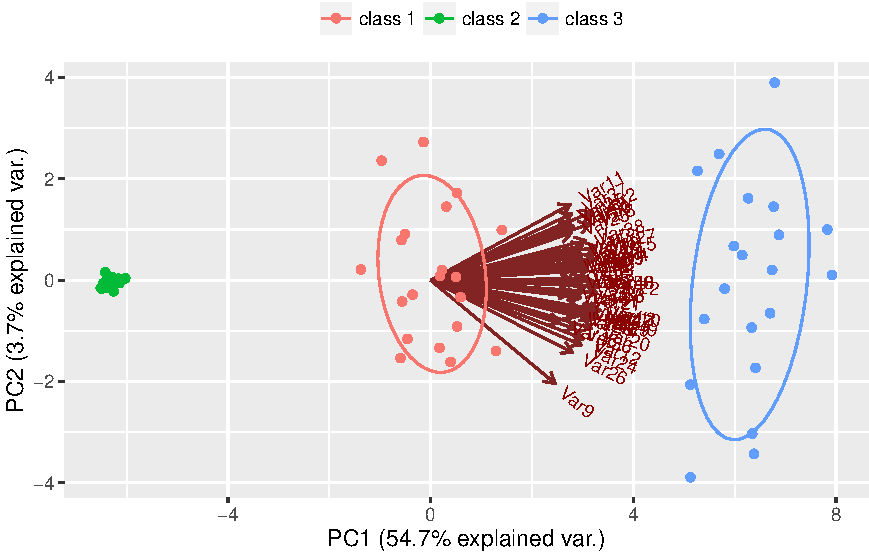
\includegraphics{sta546_hw2_files/figure-latex/unnamed-chunk-9-1.pdf}
\caption{Biplot of 3 classes groups mean shifted normally distributed
random variables}
\end{figure}

The first two principal component score vectors were plotted against one
another using our helper function \texttt{gbiplot} from Problem 1. The
\texttt{gibplot} plots the first 2 PC score vectors and uses a different
color to differentiate between the different ``classes'' of observations
(Figure 5). Figure 5 shows a good separation between the clusters of the
randomly generated classes (class 1 red cluster, class 2 green cluster,
and class 3 blue cluster). \texttt{Class 3} has the most dispersion in
the first two PCs (Figure 5).

\subsection{2.3 \textbf{K}-means clustering was conducted on the
observations with a \textbf{K} =
3}\label{k-means-clustering-was-conducted-on-the-observations-with-a-k-3}

\textbf{K}-means clustering algorithm is a popular iterative clustering
method. The algorithm is as followed (adopted from Elements of
Statistical Learning, 2e):

\begin{enumerate}
\def\labelenumi{\arabic{enumi}.}
\itemsep1pt\parskip0pt\parsep0pt
\item
  For a given cluster assignment, \(C\), the total cluster variance is
  minimized with respect to \({m_{1},...,m_{k}}\) yielding the means of
  the currently assigned clusters.
\item
  Given a current set of means \({m_{1},...,m_{k}}\) is minimized by
  assigning each observation to the closest (current) cluster mean. That
  is,
  \[C(i) = argmin_{1 \leq k \leq K} \big|\big| x_{i} - m_{k} \big|\big|^2\]
\item
  Steps 1 and 2 are iterated until the assignments do not change.
\end{enumerate}

Step 3 essentially means that steps 1 and 2 reduce the values such that
convergence is assured. This can present some problems. The convergence
may actually occurs at a local minimia along the landscape and not the
desired global minima.

\textbf{K}-means was applied to the 60 observations with \textbf{K} = 3.

\begin{Shaded}
\begin{Highlighting}[]
\NormalTok{km.k3<-}\StringTok{ }\KeywordTok{kmeans}\NormalTok{(rmat[,-}\DecValTok{51}\NormalTok{], }\DataTypeTok{centers=}\DecValTok{3}\NormalTok{) }
\KeywordTok{table}\NormalTok{(km.k3$cluster, groups)}
\end{Highlighting}
\end{Shaded}

\begin{verbatim}
##    groups
##     class 1 class 2 class 3
##   1      20      20       0
##   2       0       0      11
##   3       0       0       9
\end{verbatim}

The \textbf{K}-means algorithm was able to distinguish each of the
classes into separate clusters (class 3 in cluster 1, class 1 in cluster
2, and class 2 in cluster 3). Although the cluster number does not match
the class, the fact that it was able to correctly identify these
different classes into distinct clusters is a valid result.

\subsection{2.4 \textbf{K}-means clustering was performed with
\textbf{K} = 2 and \textbf{K} =
4}\label{k-means-clustering-was-performed-with-k-2-and-k-4}

Just as in section 2.3, \textbf{K}-means clustering was applied to the
dataset but this time with \textbf{K} = 2 and \textbf{K} = 3

\begin{Shaded}
\begin{Highlighting}[]
\NormalTok{km.k2<-}\StringTok{ }\KeywordTok{kmeans}\NormalTok{(rmat[,-}\DecValTok{51}\NormalTok{], }\DataTypeTok{centers=}\DecValTok{2}\NormalTok{)}
\KeywordTok{table}\NormalTok{(km.k2$cluster, groups)}
\end{Highlighting}
\end{Shaded}

\begin{verbatim}
##    groups
##     class 1 class 2 class 3
##   1      19       0      20
##   2       1      20       0
\end{verbatim}

The table for \textbf{K} = 2, shows that 19 observations of
\texttt{class 1} were in cluster 1 and one observation was in cluster 2.
\texttt{class 2} correctly clustered together, however, again, with 1
observation \texttt{class 1}. And lastly, all of \texttt{class 3}
clustered together in cluster 1 along with the 19 observations from
\texttt{class 1}. Intuitively, this makes sense, considering that mean
and standard deviation of the random normally distributed variables in
their (\texttt{class 1} and \texttt{class}) respective data sets are
more similar than \texttt{class 2}. So it can be expected that the
distance between \texttt{class 1} and \texttt{class 3} is less than the
distance between either class comparatively to \texttt{class 2}.

\begin{Shaded}
\begin{Highlighting}[]
\NormalTok{km.k4 <-}\StringTok{ }\KeywordTok{kmeans}\NormalTok{(rmat[,-}\DecValTok{51}\NormalTok{], }\DataTypeTok{centers=}\DecValTok{4}\NormalTok{)}
\KeywordTok{table}\NormalTok{(km.k4$cluster, groups)}
\end{Highlighting}
\end{Shaded}

\begin{verbatim}
##    groups
##     class 1 class 2 class 3
##   1      20       0       0
##   2       0       9       0
##   3       0      11       0
##   4       0       0      20
\end{verbatim}

The results for \textbf{K} = 4 show that \texttt{class 1} and
\texttt{class 2} clustered in their own clusters. \texttt{class 3} was
split into cluster 3 and 4. This may be due to the large mean and
variance of \texttt{class 3}. The \textbf{K}-means algorithm may have
classifieds the distance due to the large variance.

\subsection{2.5 \textbf{K}-means clustering was performed with
\textbf{K} = 3 on first two prinicpal component score
vectors}\label{k-means-clustering-was-performed-with-k-3-on-first-two-prinicpal-component-score-vectors}

\begin{Shaded}
\begin{Highlighting}[]
\NormalTok{km.pc <-}\StringTok{ }\KeywordTok{kmeans}\NormalTok{(}\KeywordTok{as.matrix}\NormalTok{(rmat.pc$x[,}\DecValTok{1}\NormalTok{:}\DecValTok{2}\NormalTok{]), }\DataTypeTok{centers=}\DecValTok{3}\NormalTok{)}
\KeywordTok{table}\NormalTok{(km.pc$cluster, groups)}
\end{Highlighting}
\end{Shaded}

\begin{verbatim}
##    groups
##     class 1 class 2 class 3
##   1      20       0       0
##   2       0       1      20
##   3       0      19       0
\end{verbatim}

The results reveal that when \textbf{K} = 3 was applied to the first two
PC score vectors, the classes all clustered together into their own
respective clusters. This result appears to be more accurate than just
conducting the \textbf{K}-means on the raw data. The first PC capture
most of the variance, this amount of variance must be sufficient for the
\textbf{K}-means algorithm to capture the distances from each class into
their own clusters.

\subsection{2.6 \textbf{K}-means clustering with \textbf{K} = 3 and
variables normalized to standard deviation of
1}\label{k-means-clustering-with-k-3-and-variables-normalized-to-standard-deviation-of-1}

The \texttt{stats::scale} function was applied on the data such that
each variable had a standard deviation of 1. Subsequently
\textbf{K}-means clustering with \textbf{K} = 3 was performed on the
scaled data.

\begin{Shaded}
\begin{Highlighting}[]
\NormalTok{rmat.sc <-}\StringTok{ }\KeywordTok{scale}\NormalTok{(rmat, }\DataTypeTok{center =} \OtherTok{FALSE}\NormalTok{, }\DataTypeTok{scale =} \KeywordTok{apply}\NormalTok{(rmat, }\DecValTok{2}\NormalTok{, sd))}
\NormalTok{km.sc <-}\StringTok{ }\KeywordTok{kmeans}\NormalTok{(rmat.sc, }\DataTypeTok{centers=}\DecValTok{3}\NormalTok{)}
\KeywordTok{table}\NormalTok{(km.sc$cluster, groups)}
\end{Highlighting}
\end{Shaded}

\begin{verbatim}
##    groups
##     class 1 class 2 class 3
##   1       0       0      20
##   2      20       1       0
##   3       0      19       0
\end{verbatim}

The results for 2.6 agree with the results from 2.2. In Figure 5, we can
see that from left to right, the classification of clusters goes from
\texttt{class 2} to \texttt{class 1} to \texttt{class 3}. Again the
results from 2.6 show us that \texttt{class 1} is cluster 2,
\texttt{class 2} is cluster 1, and \texttt{class 3} is cluster 3. All of
the classes were clustered into unique clusters with each of their
respective data points in \texttt{PC1} and \texttt{PC2}.

\section{Problem 3}\label{problem-3}

A gene expression data set was adopted from ISLR Ch10 Question 11. The
dataset consists of 40 tissue samples with measurements on 1,000 genes.
The first 20 samples are healthy patients and the second 20 are from a
diseased group.

\subsection{3.1 Load the data in using
\texttt{read.csv(data=Ch10Ex11.csv, header=F)}}\label{load-the-data-in-using-read.csvdatach10ex11.csv-headerf}

\begin{Shaded}
\begin{Highlighting}[]
\NormalTok{dat <-}\StringTok{ }\KeywordTok{read.csv}\NormalTok{(}\StringTok{"Ch10Ex11.csv"}\NormalTok{, }\DataTypeTok{header=}\NormalTok{F)}
\KeywordTok{colnames}\NormalTok{(dat)[}\DecValTok{1}\NormalTok{:}\DecValTok{20}\NormalTok{] <-}\StringTok{ }\KeywordTok{paste0}\NormalTok{(}\StringTok{"healthy-"}\NormalTok{, }\DecValTok{1}\NormalTok{:}\DecValTok{20}\NormalTok{)}
\KeywordTok{colnames}\NormalTok{(dat)[}\DecValTok{21}\NormalTok{:}\DecValTok{40}\NormalTok{] <-}\StringTok{ }\KeywordTok{paste0}\NormalTok{(}\StringTok{"diseased-"}\NormalTok{, }\DecValTok{1}\NormalTok{:}\DecValTok{20}\NormalTok{)}
\end{Highlighting}
\end{Shaded}

\subsection{3.2 Apply hierarchical clustering to the samples using
correlation-based distance and plot the
dendrogram.}\label{apply-hierarchical-clustering-to-the-samples-using-correlation-based-distance-and-plot-the-dendrogram.}

In comparison to the exercises that were conducted in problem 2 --
\textbf{K}-means clustering algorithms depend on the choice of
\textbf{K} (cluster centers) to be searched for and an assigned starting
point. Comparatively, hierarchical clustering methods do not require
these pre-determined conditions. Hierarchical clustering requires that
the user decides upon a measure of dissimilarity between groups of
observations, based upon the pairwise dissimilarities between the two
groups' observations.

The dissimilarity measure we chose was 1 - correlation of the raw data.
\texttt{stats::hclust} uses an agglomeration method (bottom-up) approach
for clustering. Ideally, we would like to see that the algorithm
``naturally'' represents different groups into different clusters. We
explored different types of agglomerative methods and compared them
(Figure 6). The different methods (linkage) that were chosen were: 1)
complete, 2) average, and 3) single.

\begin{Shaded}
\begin{Highlighting}[]
\NormalTok{dissimilarity <-}\StringTok{ }\DecValTok{1}\NormalTok{-}\KeywordTok{cor}\NormalTok{(dat)}
\NormalTok{dat.dist <-}\StringTok{ }\KeywordTok{as.dist}\NormalTok{(dissimilarity)}
\KeywordTok{par}\NormalTok{(}\DataTypeTok{mfrow=}\KeywordTok{c}\NormalTok{(}\DecValTok{3}\NormalTok{,}\DecValTok{1}\NormalTok{))}
\KeywordTok{plot}\NormalTok{(}\KeywordTok{hclust}\NormalTok{(dat.dist, }\DataTypeTok{method=}\StringTok{"complete"}\NormalTok{),}
     \DataTypeTok{main=}\StringTok{"Dissimilarity = 1 - Correlation (Complete Linkage)"}\NormalTok{, }\DataTypeTok{xlab=}\StringTok{""}\NormalTok{)}
\KeywordTok{plot}\NormalTok{(}\KeywordTok{hclust}\NormalTok{(dat.dist, }\DataTypeTok{method=}\StringTok{"average"}\NormalTok{),}
     \DataTypeTok{main=}\StringTok{"Dissimilarity = 1 - Correlation (Average Linkage)"}\NormalTok{, }\DataTypeTok{xlab=}\StringTok{""}\NormalTok{)}
\KeywordTok{plot}\NormalTok{(}\KeywordTok{hclust}\NormalTok{(dat.dist, }\DataTypeTok{method=}\StringTok{"single"}\NormalTok{),}
     \DataTypeTok{main=}\StringTok{"Dissimilarity = 1 - Correlation (Single Linkage)"}\NormalTok{, }\DataTypeTok{xlab=}\StringTok{""}\NormalTok{)}
\end{Highlighting}
\end{Shaded}

\begin{figure}[htbp]
\centering
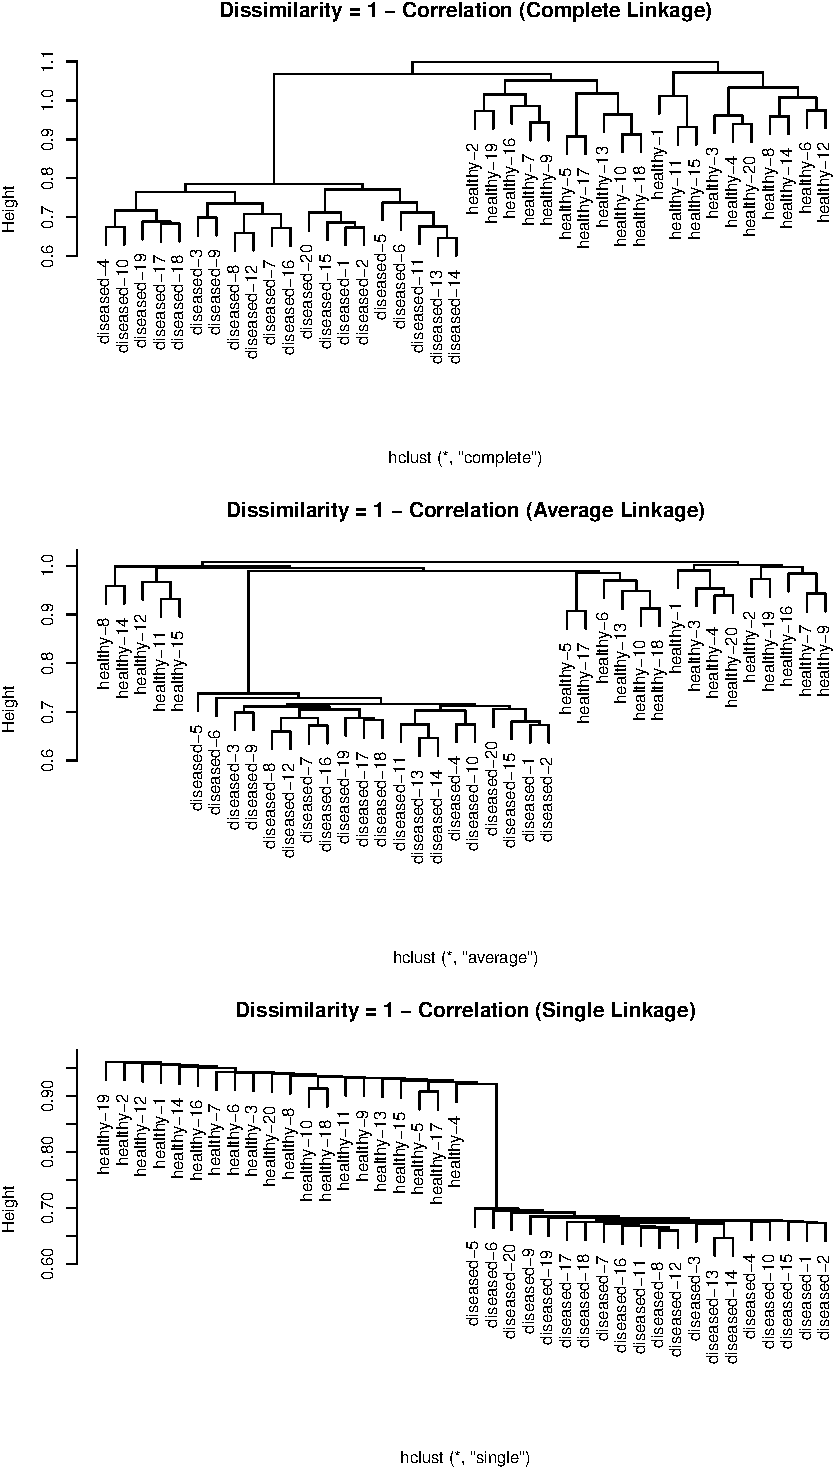
\includegraphics{sta546_hw2_files/figure-latex/unnamed-chunk-16-1.pdf}
\caption{Hiearchical Clustering With Different Linkage Methods}
\end{figure}

Looking at Figure 6 -- it seems as though using \texttt{complete}
linkage gave the best separation between the two groups.
\texttt{average} linkage seems to not do as well of job distinguishing
healthy from diseased individuals. However, \texttt{single} linkage does
separate the two groups into different clusters, but it does not appear
to be as clean as \texttt{complete} linkage.

\subsection{3.3}\label{section}

A collaborator want to know which genes differ the most across the two
groups. We can do this by doing a simple t-test or a permuted multiple
hypothesis testing t-test.

\begin{Shaded}
\begin{Highlighting}[]
\NormalTok{myttest <-}\StringTok{ }\NormalTok{function(x) }\KeywordTok{t.test}\NormalTok{(x[}\DecValTok{1}\NormalTok{:}\DecValTok{20}\NormalTok{], x[}\DecValTok{21}\NormalTok{:}\DecValTok{40}\NormalTok{])$p.value}
\NormalTok{p.val <-}\StringTok{ }\KeywordTok{apply}\NormalTok{(dat, }\DecValTok{1}\NormalTok{, myttest)}
\NormalTok{sorted_p <-}\StringTok{ }\KeywordTok{order}\NormalTok{(p.val)}
\NormalTok{dat.order <-}\StringTok{ }\NormalTok{dat[sorted_p, ]}
\NormalTok{DEgenes <-}\StringTok{ }\NormalTok{dat.order[}\DecValTok{1}\NormalTok{:}\DecValTok{100}\NormalTok{,]}
\NormalTok{DEgenes[}\DecValTok{1}\NormalTok{:}\DecValTok{5}\NormalTok{,}\DecValTok{1}\NormalTok{:}\DecValTok{5}\NormalTok{]}
\end{Highlighting}
\end{Shaded}

\begin{verbatim}
##      healthy-1   healthy-2   healthy-3  healthy-4  healthy-5
## 502 -1.2634790  0.15974770 -1.86663300 -0.8964610 -0.1393987
## 589 -0.3011929 -0.03294286 -0.82764930  0.9614763 -0.3857303
## 600  1.2134940 -0.80502150 -0.05612577 -1.4323110 -0.5125825
## 590  0.4913611 -0.61444950 -0.92325740 -0.4421924  1.3471190
## 565 -0.2453890 -0.39357150 -0.69497020  0.7439966  0.7338776
\end{verbatim}

\texttt{DEgenes} is ordered by lowest p-values from the t-test. Here we
show just the top 5 genes (indicated by row index). We would send this
list to the investigator he/she can investigate the results and gain
some biological relevance insight.

Lastly, we decided to do a permuted t-test for multiple hypothesis
testing on this data set.

\begin{Shaded}
\begin{Highlighting}[]
\KeywordTok{require}\NormalTok{(multtest)}
\NormalTok{labels <-}\StringTok{ }\KeywordTok{factor}\NormalTok{(}\KeywordTok{c}\NormalTok{(}\KeywordTok{rep}\NormalTok{(}\StringTok{"healthy"}\NormalTok{, }\DecValTok{20}\NormalTok{), }\KeywordTok{rep}\NormalTok{(}\StringTok{"diseased"}\NormalTok{, }\DecValTok{20}\NormalTok{)))}
\NormalTok{mt.test <-}\StringTok{ }\KeywordTok{mt.maxT}\NormalTok{(dat, }\DataTypeTok{classlabel=}\NormalTok{labels, }\DataTypeTok{B=}\DecValTok{10000}\NormalTok{)}
\end{Highlighting}
\end{Shaded}

\begin{verbatim}
## b=100    b=200   b=300   b=400   b=500   b=600   b=700   b=800   b=900   b=1000  
## b=1100   b=1200  b=1300  b=1400  b=1500  b=1600  b=1700  b=1800  b=1900  b=2000  
## b=2100   b=2200  b=2300  b=2400  b=2500  b=2600  b=2700  b=2800  b=2900  b=3000  
## b=3100   b=3200  b=3300  b=3400  b=3500  b=3600  b=3700  b=3800  b=3900  b=4000  
## b=4100   b=4200  b=4300  b=4400  b=4500  b=4600  b=4700  b=4800  b=4900  b=5000  
## b=5100   b=5200  b=5300  b=5400  b=5500  b=5600  b=5700  b=5800  b=5900  b=6000  
## b=6100   b=6200  b=6300  b=6400  b=6500  b=6600  b=6700  b=6800  b=6900  b=7000  
## b=7100   b=7200  b=7300  b=7400  b=7500  b=7600  b=7700  b=7800  b=7900  b=8000  
## b=8100   b=8200  b=8300  b=8400  b=8500  b=8600  b=8700  b=8800  b=8900  b=9000  
## b=9100   b=9200  b=9300  b=9400  b=9500  b=9600  b=9700  b=9800  b=9900  b=10000 
\end{verbatim}

\begin{Shaded}
\begin{Highlighting}[]
\NormalTok{sorted_mt <-}\StringTok{ }\NormalTok{dat[mt.test$index,]}
\NormalTok{sorted_mt[}\DecValTok{1}\NormalTok{:}\DecValTok{5}\NormalTok{,}\DecValTok{1}\NormalTok{:}\DecValTok{5}\NormalTok{]}
\end{Highlighting}
\end{Shaded}

\begin{verbatim}
##      healthy-1   healthy-2   healthy-3  healthy-4  healthy-5
## 502 -1.2634790  0.15974770 -1.86663300 -0.8964610 -0.1393987
## 589 -0.3011929 -0.03294286 -0.82764930  0.9614763 -0.3857303
## 600  1.2134940 -0.80502150 -0.05612577 -1.4323110 -0.5125825
## 590  0.4913611 -0.61444950 -0.92325740 -0.4421924  1.3471190
## 565 -0.2453890 -0.39357150 -0.69497020  0.7439966  0.7338776
\end{verbatim}

The multiple hypothesis testing computes an adjusted p-value, which
controls family-wise type I error (FWER). These results reveal
regardless of the controlling the FWER or not, the same genes differ the
most across the two groups.

\end{document}
